\documentclass{article}

 \usepackage{amsmath,amsfonts,
 amstext,latexsym,amssymb,amsthm,verbatim,indentfirst,alltt}
 \usepackage[pdftex]{graphicx}
 \DeclareGraphicsExtensions{.pdf,.gif,.jpg}

\newcommand{\fbold}    {\mbox{\bf f}}
\newcommand{\xbold}    {\mbox{\bf x}}
\newcommand{\Abold}    {\mbox{\bf A}}

\newcommand{\R}     {\ensuremath{\mathbb{R}}}
\newcommand{\C}     {\ensuremath{\mathbb{C}}}
\newcommand{\Q}     {\ensuremath{\mathbb{Q}}}
\newcommand{\NN}    {\ensuremath{\mathbb{N}}}
\newcommand{\Z}     {\ensuremath{\mathbb{Z}}}
\newcommand{\LL}    {\ensuremath{\mathcal{L}}}

\newcommand{\Var}   {\ensuremath{\mathrm{Var}}}
\newcommand{\spn}   {\ensuremath{\mathrm{Span}}}
\newcommand{\Tr}    {\ensuremath{\mathrm{Tr}}}
\newcommand{\diag}  {\ensuremath{\mathrm{diag}}}
\newcommand{\curl}  {\ensuremath{\nabla \times}}
\newcommand{\supp}  {\ensuremath{\mathrm{supp}}}

\newcommand{\bh}    {\backslash}
\newcommand{\nt}    {\noindent}

\newcommand{\argmin}  {\ensuremath{\operatornamewithlimits{argmin}}}


\newtheorem{alg}  {Algorithm}[section]
\newtheorem{defn} {Definition}[section]
\newtheorem{prob} {Problem}[section]
\newtheorem{thm}  {Theorem}[section]
\newtheorem{cor}  {Corollary}[section]
\newtheorem{prop} {Proposition}[section]
\newtheorem{lem}  {Lemma}[section]



\begin{document}

\title{ MATLAB Functions \\
             for
        Profiled Estimation
              of \\
       Differential Equations }

\author{Giles Hooker}

\maketitle

\tableofcontents

%\newpage

\section{Introduction}

This manual is designed to accompany a Matlab software package that estimates the parameters in
differential equation models by a profiling method.  For details on the profiling method and its
application to dynamic systems identification, see Ramsay, Hooker, Cao and Campbell (2007).  The
profiling procedure used in this package is closely related to developments in functional data
analysis described in Ramsay and Silverman (2002, 2005), and it is assumed that the user is already
reasonably familiar with this material.  Moreover, the package also makes heavy use of the Matlab
software developed by these authors, and available at the website \texttt{www.functionaldata.org}.
This software must be installed in order to use this package.

\subsection{Defining the problem}

Dynamic systems are designed to model how one or more outputs in an input/output system respond to
a change in one or more inputs. Since change is directly reflected in the derivative of an output
following the change in input, dynamic systems usually consist of a set of differential equations.
If we use the notation $x_i(t)$ to refer to the $i$th output function value at time $t$,
$i=1,\ldots,d,$ then its first derivative is denoted in various ways in the dynamic systems
literature, including $dx_i/dt$, $\dot{x}_i(t)$ and $Dx_i(t)$.  We shall use the ``dot'' notation.
If we need to refer to the vector of length $d$ containing all of the output derivatives, we use
the notation $\dot{\xbold}_i(t)$.

The functions described in this software package are designed to provide estimates of a parameter
vector $\theta$ defining an ordinary differential equation of the form:
\begin{equation} \label{de}
  \dot{x}(t) = f(t, x(t), \theta).
\end{equation}
Equation (\ref{de}) can also represent a set of $d$ coupled differential equations, and in that
case, we write
\begin{equation} \label{deindex}
  \dot{x}_i(t) = f(t, x_1(t), \ldots, x_d(t), \theta), \ i = 1, \ldots, d,
\end{equation}
or more compactly in matrix notation
\begin{equation} \label{devec}
  \dot{\xbold(t)} = \fbold(t, \xbold(t), \theta).
\end{equation}

The right hand function $f$ defines the functional relationship of change, expressed as
$\dot{x}(t)$, to:
\begin{itemize}
  \item $x$ itself,
  \item time $t$ in ways other than through the value $x(t)$ and
  \item a vector of parameters $\theta$ whose values must be estimated in order to completely
  define the dynamic system.
\end{itemize}
It is frequently the case that the dependency on time $t$ other than via $x(t)$ is through one or
more input functions $u_{i\ell}, \ell = 1,...,L_i$.  In this case, these input functions are often
referred to as \emph{forcing} functions that are said to \emph{force} the specific equation(s)
affected by them, and (\ref{de}), for example, can also be written as
\begin{equation} \label{deforce}
  \dot{x}(t) = f(x(t), u(t), \theta).
\end{equation}

For a specific example of a dynamic system, see (\ref{FhNequations}) defining the FitzHugh-Nagumo
equations in the next section.

We assume that we have noisy data
\[
  y_i(t_{ij}) = x_i(t_{ij}) + \epsilon_{ij}, j=1,\ldots,n_i,
\]
and that we wish to use these data to estimate  $\theta$. The measurement times $t_{ij}$ may not be
the same for all of the variables $y_i$, and the standard deviations, $\sigma_i$, of the
measurement errors $\epsilon_{ij}$ may also vary. This software has been produced to take these
aspects of the data into account.

More generally, however, the derivatives need not necessarily be of the order 1. That is, the order
$m$ of equation $i$, being the order of the highest derivative involved in the equation, may vary
from equation to equation, and may also be 0.  In particular, a zero'th order derivative for some
component corresponds to an Algebraic Equation.  Right side function $f$ may also incorporate
derivatives of $x(t)$, and delayed evaluation, $x(t-\delta)$. While the initial presentation of the
software here will assume a set of first order ordinary differential equations, Section
\ref{example2} will demonstrate the application of this software to equations of varying orders.

\subsection{The profiling estimation procedure}

The profiling estimation procedure used by this software has two stages of optimization, which we
will label the {\em inner} and {\em outer} stages. Each of these stages is associated with its own
unique fitting criterion.

\subsubsection{The basis function expansion of $x_i$:}

We approximate each $x_i$ by a basis function expansion,
\[
  \hat{x_i}(t) = \sum_{k=1}^{K_i} c_{ik} \phi_{ik}(t),
\]
where$\phi_{ik}(t)$ is a specific basis function in the basis system used for variable $i$, and the
coefficients $c_{ik}$ are estimated from the data so as to provide an optimal fit.  Note that the
nature and number of basis functions can vary from one variable to another.  Ramsay and Silverman
(2005) can be consulted for advice on how to choose a basis function system.

\subsubsection{The inner optimization:}

In the inner stage, the equation parameter vector $\theta$ is kept fixed, and it is the basis
expansion coefficients $c_{ik}$ that are estimated.  This in turn estimates a vector of smooth
functions, $\hat{x}_i$.  We can, if we wish, emphasize that the fit in the inner stage depends on
the value of parameter vector $\theta$ by using the notation $\hat{x}_i(t|\theta)$.

The data are fit by minimizing the penalized sum of squares
\begin{equation} \label{spline}
 G(x,\theta,\lambda) = \sum_{i=1}^n \left\{ \|y_i - x_i(t_i)\|^2 +
       \lambda_i \int \left( \dot{x}_i(t) - f_i(t,x(t),\theta) \right)^2 dt \right\},
\end{equation}
where $y_i$ and $t_i$ are intended to indicate the vectors of measured values and measuring times
for the $i$th variable, respectively. The norm notation $\| \cdot \|^2$ is used here to represent a
sum of squared error measure of fit of the estimated variable values to their respective data.
Varying weights for each squared error are permitted.

The second term in this equation specific to variable $i$ measures the fidelity of $\hat{x}_i$ to
the differential equation specific to that variable. The fit measure in this second term is also a
least squares measure, but the summation over discrete values $t_i$ of $t$ in the first term has
been replaced an an integration over the continuum of $t$ values. We approximate the integral in
(\ref{spline}) by a numerical quadrature method whose accuracy can be controlled by the user of the
software package.

A smoothing parameter $\lambda_i$ trades-off fidelity to the equations and to the data for variable
$i$. When $\lambda_i$ is near zero, the second term in (\ref{spline}) has little impact on the fit,
and we are consequently smoothing the data with little regard for whether the smooth satisfies the
differential equation for that variable.  However, when $\lambda_i$ is large, the second term tends
to dominate the criterion (\ref{spline}), and consequently $\hat{x}_i$ is forced to closely satisfy
the differential equation, with the fit to the data being as good as possible given this
constraint. If we use the notation $x_{t|\theta}$ as an estimate of the true trajectory, or path,
that the system took, then we see that the composite fitting criterion (\ref{spline}) allows for
some discrepancy between an exact solution to the differential equation\ref{de} and the estimated
fit $\hat{x}_i$. In this way we can accommodate modeling situations in which the equation is known
to only provide an approximate model of the actual dynamic system giving rise to the data.

Because we use a quadrature rule to approximate the integrals in (\ref{spline}), each second term
is also essentially an error sum of squares. Consequently, the total fit measure (\ref{spline}) can
now be re-expressed as a non-linear least-squares problem, and the Gauss-Newton algorithm is
employed in our software to actually carry out the inner optimization.

\subsubsection{The outer optimization:}

The parameters in vector $\theta$ are varied in the outer optimization, and are required to
minimize the outer criterion:
\begin{equation} \label{parest}
  J(\theta,\lambda) = \sum_{i=1}^n \|y_i - x_i(t_i|\theta)\|^2,
\end{equation}
which measures only the squared distance between the data and the smooth.  We use the notation
$x_i(t_i|\theta)$ to stress that the fit to variable $i$ in this stage is actually a
\emph{function} of $\theta$, since it is re-estimated \emph{each} time $\theta$ is changed.  This
functional relationship is what is implied by the term \emph{profiling}.

Note that the outer criterion lacks the fidelity-to-equation terms in (\ref{spline}).  These are no
longer needed, since the functional relationship that profiling implies ensures that the fit will
always be smoothed at a level defined by the value of $\lambda_i$.  There is no need to penalize
the roughness of $\hat{x_i}$ twice.

We can also solve (\ref{parest}) via another Gauss-Newton procedure, making use of the derivative
\[
  \frac{dJ}{d\theta} = \frac{dJ}{dc} \frac{dc}{d\theta},
\]
where
\[
  \frac{dc}{d\theta} = - \left[ \frac{d^2G}{dc^2} \right]^{-1} \frac{d^2G}{dcd\theta}
\]
by the Implicit Function Theorem.

The rest of this document describes how to get this software to do this by making use of the
Functional Data Analysis (FDA) software package for MATLAB.

\section{Example: FitzHugh-Nagumo Equations}

Throughout this document, we will use the FitzHugh-Nagumo equations as an example. These relatively
simple equations are widely used in modeling neuro-physiological processes, and a discussion of the
historical development of these equations as well as many applications can be found in Beuter,
Glass, Mackey and Titcombe (2003). The equations are
\begin{eqnarray} \label{FhNequations}
  \dot{V} & = c \left( V - \frac{V^3}{3} + R \right) \\
  \dot{R} & = -\frac{1}{c} \left( V -a + bR \right),
\end{eqnarray}
with the $\theta = \{a,b,c\}$ being the unknown parameter vector, variable $V$ being the voltage
across the cell boundary and $R$ representing a set of recovery processes. If we use the notation
in (\ref{de}), these equations are
\begin{eqnarray} \label{FhNequations2}
  \dot{x}_1 & = c \left( x_1 - \frac{x_1^3}{3} + x_2 \right) \\
  \dot{x}_2 & = -\frac{1}{c} \left( x_1 -a + bx_2 \right).
\end{eqnarray}
and we could also use an algebraic equation to write them as
\begin{eqnarray} \label{FhNequations2}
  \dot{x}_1 & = c \left( x_1 - \frac{x_3}{3} + x_2 \right) \\
  \dot{x}_2 & = -\frac{1}{c} \left( x_1 -a + bx_2 \right) \\
  x_3       & = x_1^2.
\end{eqnarray}

A plot of solutions to these equations is given below for parameter values $\{0.2,0.2,3\}$ and
initial conditions $[x_1(0),x_2(0)] = [-1,1]$.

\begin{center}
%  \includegraphics[height=5cm]{est_figs/fhn_paths.png}
  \includegraphics[height=5cm]{figs/fhn_paths.png}
\end{center}

\section{MATLAB Objects Needed for the Estimation. }

\subsection{Cell Arrays}

The software works uses Matlab cell arrays to contain information about each variable, since the
nature an amount of information can vary from variable to variable. That is, the contents of each
cell in a cell array corresponds to one variable $x_i$ of the system. When the system is observed
only once, these arrays take the form of a {\em row vector}; one element of the row representing
one variable of the system. For example, the two equations in the FitzHugh-Nagumo equations above
appear in the first and second cells in a cell array defined by a Matlab command such as
\texttt{FHcell = cell(1,2)}, respectively.

When a system has been observed a number of times, each replication is represented by the
corresponding row of a two-dimensional array. The description of the system used here will assume
data {\em without} replications. Section \ref{replications} will introduce the modifications
necessary to estimate equations with replicated data.

When there are individual numbers which correspond to variables of a system -- for example, the
smoothing parameters, $\lambda$ or the variable weights $w_i$ -- these may be represented by a
regular numeric array rather than a cell-array.

The use of cell arrays is detailed in standard MATLAB manuals, but because of the heavy reliance of
this code on them, a quick review of the basics is given below. Cell arrays behave like standard
arrays, except that each component may contain an arbitrary MATLAB object. In our case, they will
be used to store estimated paths and bases.

Cell arrays are indexed in the same manner as standard arrays. The crucial distinction is that
assigning content to arrays makes use of curly braces. Enclosing a vector of objects in curly
braces denotes a cell array containing those objects, thus

\begin{alltt}
    A = cell(1,2);
\end{alltt}

\nt which creates a 1 by 2 array of empty cells, is equivalent
to

\begin{alltt}
    A = \{[], []\}.
\end{alltt}

\nt Similarly, calling content from a cell array requires curly
braces so that

\begin{alltt}
    A(1,1)
\end{alltt}

\nt returns a 1 by 1 cell array containing an empty object,
whereas

\begin{alltt}
   A\{1,1\}
\end{alltt}

\nt returns the empty object with {\tt A} defined above. Note that

\begin{alltt}
   A(1:2)
\end{alltt}

\nt is legitimate notation in MATLAB, but

\begin{alltt}
   A\{1:2\}
\end{alltt}

\nt is not. A final shortcut that we make use of is to
allow the entries in a cell array to be replicated, so that
to insert 0 as the content of both entries of {\tt A} we
can either set

\begin{alltt}
   A(1:2) = \{0,0\}
\end{alltt}

\nt or

\begin{alltt}
   A(1:2) = \{0\}.
\end{alltt}

\nt Note that

\begin{alltt}
   A\{1:2\} = 0
\end{alltt}

\nt will produce an error.

\subsection{Data Objects}

\nt The raw data supplied to the estimation scheme is stored in two cell arrays:
\begin{description}
\item[\tt Tcell:] the times at which the variable of the system
is measured.
\item[\tt Ycell:] the values measured at the times in {\tt Tcell}.
\end{description}
As indicated above, the columns of these cell arrays correspond to variables and the rows to
replications, and each cell contains a vector of values.  Of course, the number of times values in
a specific cell in \texttt{Tcell} must equal the number of variable values in the corresponding
cell in \texttt{Ycell}, but may vary from one variable to another.

\nt We will use simulated data to demonstrate the system in action. To do this, we require data in
an object {\tt path\_cell}, which we set up as follows:

\begin{alltt}
    Tcell = \{0:0.05:20, 0:0.05:20\};
    path = ode45(@fhnfunode,0:0.05,20,[-1,1],[],[0.2 0.2 3]);
    path_cell = \{path(:,1), path(:,2)\}
\end{alltt}

\nt which produces the paths plotted above.  The function
{\tt fhnfunode} calculates the right-hand side of the
FitzHugh-Nagumo equations for a given vector of inputs and
{\tt ode45} is a Runge-Kutta solver for differential
equations in MATLAB. From this, we can create data by
adding noise to the FitzHugh-Nagumo path:

\begin{alltt}
  Ycell = path_cell;
  for(i = 1:length(path_cell))
    Ycell\{i\} = path(:,i) + 0.5*randn(size(path,1),1);
  end
\end{alltt}

Note that some elements of {\tt Tcell} and {\tt Ycell} may be left as empty cells. These represent
unmeasured variables of the system. {\tt Tcell} may also be given as a simple vector, in which case
all variables of the system are assumed to be measured at the same times.


\subsection{Basis Objects} \label{fd_objs}

We represent the smooth $x_j$ for each variable of $x$ by a functional data object stored in a cell
array. Each variable may be represented by a different basis system. However, it is expected that
each basis will cover the same range and will use the same quadrature points. For a cell-array of
basis objects, {\tt basis\_cell}, the function

\begin{alltt}
   checkbasis(basis_cell)
\end{alltt}

\nt will verify that all the bases have the same range.
This should not be necessary if {\tt basis\_cell} is set up as
follows.

For ease of use, a function {\tt MakeQuadPoints} is available:

\begin{alltt}
   quadvals = MakeQuadPoints(knots,nquad)
\end{alltt}

\nt where {\tt knots} is the set of all knots used in B-spline bases across all variables of the
system and {\tt nquad} is the number of quadrature points to place between knots. This sets up
equally spaced quadrature points on these knots and associates Simpson's rule quadrature values
with them.

A B-spline basis using these quadrature points can be set
up via the function

\begin{alltt}
basis_obj = MakeBasis(range,nbasis,norder,knots,quadvals,nderiv);
\end{alltt}

\nt with the following inputs

\begin{description}
    \item[range:] the range of the basis
    \item[nbasis:] the number of basis functions to use
    \item[norder:] the order of the basis functions
    \item[knots] the knots to use
    \item[quadvals:] as above, quadrature points and values
    \item[nderiv:] the number of derivatives at which a
    functional data object is expected to be evaluated.
    This should be the same as the maximum number of
    derivatives appearing in (\ref{de}).
\end{description}

We have found that good smooths can require very
large numbers of basis functions. However, the order of the
B-spline does not seem to affect the quality of the smooth
and the minimum value for {\tt nquad}, 5, appears
to be sufficient. Usually, only the functional data objects
and their first derivatives will need to be evaluated.

The following code sets up basis functions for each of the variables in the FitzHugh-Nagumo
equation example:

\begin{alltt}
    knots = 0:0.5:20;
    quadvals = MakeQuadPoints(knots,5);

    norder = 3;
    nbasis = length(knots) + norder - 2;
    basis_obj = MakeBasis([0 20],nbasis,norder,knots,quadvals,1);
    basis_cell = \{basis_obj, basis_obj\};
\end{alltt}

\subsection{Functional Data Objects}

In order to perform the non-linear least squares estimation
for the coefficient vectors of these basis functions,
initial values need to be provided. They can be set to
zero, but it may be advantageous to estimated these by a smooth
using a first-derivative penalty. The function {\tt
smoothfd\_cell} provides a wrapper to {\tt smoothfd} to loop
over the values in a cell-array of objects:

\begin{alltt}
   lambda0 = 0.1;
   Lfd_cell = cell(size(basis_cell));

   for(i = 1:length(basis_cell))
     fdPar_cell\{i\} = fdPar(basis_cell\{i\},1,lambda0);
   end

   DEfd = smoothfd_cell(Ycell,Tcell,fdPar_cell);
\end{alltt}

\nt When some elements of {\tt Tcell} are empty, the coefficients of that variable are estimated as
zero. This does not always provide great results and some other initial conditions may be helpful.
This might include simply using a nonzero constant. Other possibilities are discussed in Section
\ref{mod-smooth}.

{\tt DEfd} is now the cell array of functional data objects
that we want. For the purposes of smoothing, we need the
coefficients of these objects. In this case

\begin{alltt}
   coefs = getcellcoefs(DEfd);
\end{alltt}

\nt provides these as a single vector concatenated from
all the coefficients vectors. This can then be used as an
argument to {\tt lsqnonlin} as detailed in Section
\ref{estimation}.

\subsection{Weights and Smoothing Parameters}

\nt Two further objects are needed:

\begin{description}
\item[lambda] defines the smoothing parameter to use in
(\ref{spline}). It may be a vector, defining one parameter for each variable of the system. If a
singleton, it is assumed to be the same for every variable.

\item[wts] defines a weight for each observation. It may be
empty (each observation gets the same weight), a vector (giving a different weight to each variable
of the system, but the same weight within a variable) or a cell array (defining a different weight
for each observation).
\end{description}

The variable weights in vector {\tt wts} should be inversely proportional to the size of
measurement noise in each variable. Alternatively, we might weight by the simple variance in each
variable.

The smoothing or bandwidth parameter values in vector \texttt{lambda} control the extent to which
each estimated variable satisfies it's corresponding differential equation.  If $\lambda_i$ is
relatively close to zero, the estimated variable $\hat{x}_i$ will only be lightly constrained by
the differential equation, and will primarily smooth the data.  For difficult problems having
complex fitting surface topology when the equations are closely satisfied (as is the case for the
FitzHugh-Nagumo equations) small values in \texttt{lambda} are advisable in the initial stages of
parameter estimation, followed by increasing them incrementally until the desired fidelty to the
equation has been attained.

The setting up of \texttt{wts} and \texttt{lambda} is illustrated in the following code:

\begin{alltt}
   lambda = 1000*ones(size(DEfd));

   wts = zeros(size(DEfd));
   for(i = 1:length(DEfd))
     wts(i) = 1/sqrt(var(Ycell{i}));
   end
\end{alltt}

\section{Defining the Differential Equation}

\subsection{Derivatives on the Left Hand Side}

The left hand side requires a vector {\tt alg} to be specified giving the order of derivative to be
used in each variable of the system. This is a vector of non-negative integers of the same length
as the system, specifying the order of each differential equation.

Usually, as in the case of the FitzHugh-Nagumo equations,
this is simply

\begin{alltt}
   alg = [1 1];
\end{alltt}

\nt but algebraic equations may be specified by setting the corresponding variables of {\tt alg} to
zero. Higher-order equations may be specified by correspondingly higher entries in {\tt alg}. An
example of using algebraic and higher order terms is given in Section \ref{example2}.

If {\tt alg} is left empty, it is assumed to
be a vector of ones.

\subsection{Functions for the Right Hand Side}

The estimation procedure requires the user to write functions to compute $f(t,x,\theta)$ and
several of its derivatives. All these functions take the one of the two following two forms

\begin{alltt}
   fn(t,DEfd,pars)
\end{alltt}

or

\begin{alltt}
   fn(t,DEfd,pars,moreinfo)
\end{alltt}

\nt where {\tt t} is a vector of times at which to evaluate the function and {\tt pars} is the
vector of parameter estimates. The fourth argument {\tt moreinfo} in the second form may be
required to contain any extra input into the function, such as information on forcing functions.
The form of this input is left up to the user, but would typically be a struct object with fields
containing additional required quantities.

The output of each required function should be a cell-array of values. The number of dimensions of
the cell array will depend on whether the function values only are computed, the partial
derivatives with respect to $x$, and/ or the partial derivatives with respect to $\theta$. The
total number of dimensions is  \#(no. derivatives)+1. The first dimension is determined by the
function values, the second by the $x$-derivatives if computed, then followed by the
$\theta$-derivatives if computed.  That is, the variables of $F$ are in the first dimension with
the derivatives in the following dimensions. Derivatives with respect to variables of $x$ will
always be taken before derivatives with respect to variables of $\theta$. The elements of these
cell arrays will be time series corresponding to the evaluation of the relevant variable and
derivative at the smooth {\tt DEfd} evaluated at times {\tt t}.  See below for illustrations of
this output organization.

To aid in writing these functions, a wrapper function {\tt
  eval\_fdcell} is provided

\begin{alltt}
   fvals = eval_fdcell(Tcell,DEfd,deriv)
\end{alltt}

\nt where {\tt Tcell} is either a cell-array or a vector (implicitly made
into a cell-array all elements containing the vector) of time points
at which to evaluate {\tt DEfd} and {\tt deriv} is the order of
derivative to take and may be a vector so that

\begin{alltt}
   eval_fdcell(Tcell,DEfd,0)
\end{alltt}

\nt provides the values of DEfd at the observation times and

\begin{alltt}
   eval_fdcell(0:20,DEfd,1)
\end{alltt}

\nt provides the first derivatives of DEfd at unit time intervals. The
output from these are, of course, cell arrays.

The organization of the output of the functions is illustrated in the following examples for the
FitzHugh-Nagumo equations.

Thus, the function defining the right hand side of the FitzHugh-Nagumo
equations will be given by a MATLAB file containing ({\tt
p} is substituted for $\theta$ throughout the code):

\begin{alltt}
   function r = fhnfun(t,DEfd,p)

   x = eval_fdcell(t,fd_cell,0);
   r = x;
   r\{1\} = p(3)*(x\{1\} - x\{1\}.^3/3 + x\{2\});
   r\{2\} = -(x\{1\} -p(1) + p(2)*x\{2\})/p(3);

   end
\end{alltt}

\nt the derivative of $f$ with respect to the parameters is

\begin{alltt}
   function r = fhndfdp(t,DEfd,p)

   x = eval_fdcell(t,fd_cell,0);
   r = cell(2,3);

   r(1:2,1:3) = \{0\};

   r\{1,3\} =  (x\{1\}-x\{1\}.^3/3+x\{2\});
   r\{2,1\} = 1/p(3);
   r\{2,2\} = (-x\{2\}/p(3));
   r\{2,3\} = ((x\{1\}-p(1)+p(2)*x\{2\})/(p(3).^2));

   end
\end{alltt}

\nt and the second derivative with respect to $x$ and $\theta$ is

\begin{alltt}
   function r = fhnd3fdxdp(t,DEfd,p)

   r = cell(2,2,3);
   r(1:2,1:2,1:3) = \{0\};

   r\{1,1,3\} = 1 - eval_fd(t,fd_cell{1}).^2;
   r\{1,2,3\} = 1;
   r\{2,1,3\} = 1/p(3)^2;
   r\{2,2,2\} = - 1/p(3);
   r\{2,2,3\} = p(2)/p(3)^2;

   end
\end{alltt}

\nt Where a derivative is constant, a simple number can be returned in
the corresponding cell and this will save some computation.

In order to perform the profiled estimation scheme, a total of five
functions are required:

\[ f, \ \frac{df}{dx}, \ \frac{df}{d\theta}, \ \frac{d^2f}{dx^2}, \
\frac{d^2f}{dxd\theta}. \]

\nt If variance estimates are required for the parameters, a further
four functions are needed:

\[ \frac{d^2f}{d\theta^2}, \ \frac{d3f}{dx^3}, \ \frac{d3f}{dx^2d\theta}, \
\frac{d3f}{dxd\theta^2}. \]

Note that although the examples above are given for an ODE, these functions may also incorporate
evaluating derivatives of {\tt DEfd} and evaluating variables of {\tt DEfd} at lagged intervals.

The estimation code expects these functions to be given
in a struct whose elements are function handles with fields specified
in the following manner:

\begin{alltt}
   fn.fn       = @fhnfun;       \% RHS function
   fn.dfdx     = @fhndfdx;      \% Derivative wrt inputs (Jacobian)
   fn.dfdp     = @fhndfdp;      \% Dervative wrt parameters
   fn.d2fdx2   = @fhnd2fdx2;    \% Hessian wrt inputs
   fn.d2fdxdp  = @fhnd2fdxdp;   \% Hessian wrt inputs and parameters
   fn.d2fdp2   = @fhnd2fdp2;    \% Hessian wrt parameters.
   fn.d3fdx3   = @fhnd3fdx3;    \% 3rd derivative wrt inputs.
   fn.d3fdx2dp = @fhnd3fdx2dp;  \% 3rd derivative wrt intputs and pars.
   fn.d3fdxdp2 = @fhnd3fdxdp2;  \% 3rd derivative wrt inputs and pars.
                                \% dimensions = time, variable, input,
                                \% parameters
\end{alltt}

\nt and the struct {\tt fn} can now be used as an input
into any of the estimating functions.


\section{Calling Estimation Functions}  \label{estimation}

The software carries out two tasks. The inner optimization of $G(x,\theta,\lambda)$ defined in
(\ref{spline}), equivalent to conducting a model-based smooth, and an outer optimization
$J(\theta,\lambda)$, or choosing the parameters that optimize the smooth.

\subsection{Model-Based Smoothing} \label{mod-smooth}

\nt The set of coefficients minimizing (\ref{spline}) can be obtained by a
call to the MATLAB routine {\tt lsqnonlin} to optimize

\begin{alltt}
  SplineCoefErr(coefs,basis_cell,Ycell,Tcell,wts,lambda,...
      fn,alg,pars,moreinfo)
\end{alltt}

\nt Here {\tt SplineCoefErr} calculates the value of
$G(x,\theta,\lambda)$, along with its derivative with
respect to the coefficients defining the smooth
$x_{\theta}$.

Array {\tt coefs} may be obtained as in \S\ref{fd_objs} and array{\tt pars} contains the parameters
$\theta$. Struct object {\tt fn\_extras} is an optional extra argument that contains any additional
information required to compute the right hand side and its derivatives, and does not needed to be
included in the function call if no additional information is required. All other inputs are as
given in the above sections.

In the case of the FitzHugh-Nagumo example, we would call {\tt
  lsqnonlin} as follows:

\begin{alltt}
   coefs = lsqnonlin(@SplineCoefErr,coefs,[],[],[],basis_cell,...
       Ycell,Tcell,loads,lambda,fn,alg,pars);
\end{alltt}

\nt the cell array of functional data objects can then be recovered by

\begin{alltt}
   DEfd = Make_fdcell(coefs,basis_cell);
\end{alltt}

\nt As an alternative, the function

\begin{alltt}
   DEfd = SplineEst(fn,Tcell,Ycell,pars,knots_cell,wts,...
        lambda,lambda0,rough_ord,alg,lsopts,DEfd,moreinfo);
\end{alltt}

\nt provides a wrapper for the call to {\tt lsqnonlin}. It defines a basis using the knots
specified in {\tt knots\_cell} (again, one set of knots per variable of $x$, but this may be a
vector which will then be replicated across all variables), and creates an initial smooth defined
by {\tt lambda0} and the roughness penalty specified by the {\tt Lfd} object {\tt rough\_ord}.

{\tt lsopts} are the optimization options to be
passed to {\tt lsqnonlin}. If the functional data object cell
array {\tt DEfd} is not empty, this is passed directly to {\tt
  lsqnonlin} without defining a new cell array of bases.

We could alternatively create {\tt DEfd} this smooth by the
call:

\begin{alltt}
   DEfd = SplineEst(fn,Tcell,Ycell,[0.2 0.2 3],...
        0:0.05:20,wts,1000,0.1,1,[],[],[],[]);
\end{alltt}

This routine may not always give good results when unmeasured variables are poorly specified, or
when there is relatively little data. Section \ref{variations} details a function that will
estimate unmeasured variables from the others, using the differential equation.  Possibly the best
solution is to smooth the data with the differential equation using a small value of $\lambda$ and
using this as initial conditions with a larger $\lambda$. This scheme may need to be iterated a few
times to achieve an appropriate amount of smoothing.



\subsection{Profiled Estimation}

The profiled estimation routine to estimate $\theta$ uses its own
Gauss-Newton iteration scheme. This allows {\tt DEfd} to be updated
along with {\tt pars}, providing some computational speedup. The
routine is called by

\begin{alltt}
   [newpars,DEfd] = Profile_GausNewt(pars,lsopts,DEfd,fn,...
            lambda,Ycell,Tcell,wts,alg,lsopts2,moreinfo,...
            pen,dpen,pen_extras);
\end{alltt}

\nt here {\tt lsopts} and {\tt lsopts2} are optimization options to
the outer and inner minimization routines respectively. They follow
exactly the optimization toolbox options and may be set with the
MATLAB {\tt optimset} command. As in model based smoothing, {\tt
  fn\_extras} does not needed to be included in the function call
  if these two arguments are empty.

Finally, it is possible that we may wish to modify the
outer criterion to

\[ \tilde{J}(\theta,\lambda) = J(\theta,\lambda) +
P(\theta) \]

\nt in which $P(\theta)$ regularizes the estimated values
of $\theta$. This will be the case if, for instance,
$\theta$ is high dimensional. This might occur, for
example, if they are taken to be coefficients of a basis
expansion for a functional parameter.
The entries {\tt pen}, {\tt dpen} and {\tt
pen\_extras} define such penalties on the parameters.
{\tt pen} and {\tt dpen} should be functions accepting
{\tt pars} and {\tt
pen\_extras} and outputting a vector giving the penalty (to
be squared) and it's derivative respectively.

This separate Gauss-Newton optimization routine has been
employed so that the object {\tt DEfd} may be updated as
the optimization progresses. Whenever we update $\theta$,
the coefficients $c$ will also be updated, and their new
values can be anticipated by using $dc/d\theta$.


\nt For the FitzHugh-Nagumo equations, the call becomes

\begin{alltt}
 lsopts_out = optimset('DerivativeCheck','off','Jacobian','on',...
   'Display','iter','MaxIter',maxit0,'TolFun',1e-8,'TolX',1e-10);

 lsopts_in = optimset('DerivativeCheck','off','Jacobian','on',...
     'Display','off','MaxIter',maxit1,'TolFun',1e-14,...
     'TolX',1e-14,'JacobMult',@SparseJMfun);

 [newpars,newDEfd] = Profile_GausNewt(pars,lsopts_out,DEfd,fn,...
     lambda,Ycell,Tcell,wts,alg,[],[],[],lsopts_in);
\end{alltt}

\nt Note that an initial guess for {\tt pars} is necessary to start the
minimization.

\section{Covariance Matrices of Parameter Estimates} \label{covariance}

A covariance matrix may be calculated for the parameter estimates via
a $\delta$-method:

\[ \Var(\theta) \approx \frac{d \theta}{dx}^T \Var(y) \frac{d
  \theta}{dx} \]

\nt where

\[ \frac{d \theta}{dx} = - \left[\frac{d^2J}{d\theta^2}\right]^{-1}
\frac{d^2J}{d\theta dY} \]

\nt These two matrices, along with $\Var(y)$, must be calculated individually.

\nt $d^2J/d\theta^2$ is calculated using the following function:

\begin{alltt}
   d2Jdp2 = make_d2jdp2(DEfd,fn,Tcell,lambda,pars,alg,wts,...
       Ycell,moreinfo,d2pen,pen_extras)
\end{alltt}

\nt where {\tt d2pen} is a function providing the second
derivative of a penalty with respect to parameters. It
takes the same arguments as {\tt pen} and {\tt dpen} in
\\ {\tt Profile\_GausNewt}.

$d^2J/d\theta dx$ is calculated by the following

\begin{alltt}
   d2Jdpdy = make_d2jdpdY(DEfd,fn,Tcell,lambda,pars,alg,wts,...
      Ycell,moreinfo)
\end{alltt}

\nt and $\Var(y)$ is a diagonal matrix calculated in

\begin{alltt}
    S = make_sigma(DEfd,Tcell,Ycell,ind)
\end{alltt}

\nt where {\tt ind} indicates the method used to calculate the variance of the observational noise.
A value of 0 indicates that all variables have an individual variance, 1 indicates pooling across
replicates but within variables, 2 pooling across variables within replicates and 3 pooling across
all variables. These should be chosen according to the system. It is most likely that 0 or 1 will
be appropriate -- this will be especially true when different variables are measured in different
units. However, when different variables share the same scales and measurement accuracy, using
options 2 or 3 will stabilize the variance estimate.

A covariance matrix for the parameter estimates for the
FitzHugh-Nagumo equations can now be calculated by

\begin{alltt}
   d2Fdp2 = make_d2jdp2(newDEfd_cell,fn,Ycell,Tcell,lambda,...
       newpars,alg,wts)

   d2FdpdY = make_d2jdpdy(DEfd,fn,Ycell,Tcell,lambda,newpars,...
       alg,wts);

   dpdY = -d2Fdp2\(\bh\)d2FdpdY;

   S = make_sigma(DEfd,Tcell,Ycell,0);

   Cov = dpdY * S * dpdY'
\end{alltt}


\section{Parameter Estimation with Replication} \label{replications}

In some cases, more than one time series corresponding to a system of
differential equations may be observed. Moreover, it is possible that
only some of the parameters will be common to different replications
of the system.

Where replicates of the system are measured, the cell arrays, {\tt
  Tcell}, {\tt Ycell}, and {\tt DEfd} now become cell matrices
with rows representing replications and variables given in columns. The bases for different
replications do not need to share the same range or quadrature points.

In order to estimate parameters for such systems, new functions need
to be used for those in \S\ref{estimation} and
\S\ref{covariance}. These take the same arguments as their
single-replicate counterparts with the additional input of

\begin{description}
\item[parind] a matrix whose rows give the indices of the entries of the
  parameter vector that correspond to parameters for each replicate.
\end{description}

\nt The use of {\tt parind} allows some parameters to be shared and
others estimated separately. For instance, if, in the FitzHugh-Nagumo
equations, parameters $a$ and $b$ were shared between two replicates,
but $c$ was not, we would define the following

\begin{alltt}
   pars = [a b c1 c2];

   parind = [1 2 3;
             1 2 4];
\end{alltt}

\nt if {\tt parind} is left empty, the code uses a default
that all parameters are common to all replications.

 The input {\tt parind} follows {\tt pars} in each of the
functions, {\tt SplineCoefErr\_rep}, {\tt Profile\_GausNewt\_rep}, {\tt
  make\_d2jdp2\_rep} and {\tt make\_d2jdpdy\_rep}. These may all be used
with single-replicate systems as well.
{\tt make\_sigma} already incorporates replications.


\section{Estimating Starting Values from a Smooth} \label{variations}

This section details two functions that will provide estimates for unmeasured variables of a system
and initial parameter values respectively. We assume that all variables have been estimated by a
smooth of the data using, say, a first-derivative penalty.

\subsection{Unmeasured Variables}

Suppose that we have derived {\tt DEfd} from a call to {\tt smoothfd\_cell} which has set some
unmeasured variables to be zero. If we desire a better initial estimate, we could treat the smooths
for the measured variables of {\tt DEfd} as fixed, and then try to find coefficients for the
unmeasured variables that best fit the differential equation.

The following function can be optimized with {\tt lsqnonlin}:

\begin{alltt}
   SplineCoefErr_DEfit(coefs,DEfd,ind,fn,pars,alg,moreinfo)
\end{alltt}

\nt Here {\tt ind} gives the indices of the unmeasured variables, {\tt coefs} is a single vector
giving initial estimates of the coefficients for the variables listed in {\tt ind}. {\tt DEfd} is
the fit from the smooth, {\tt pars} are guesses at the parameters and {\tt fn}, {\tt alg} and {\tt
fn\_extras} are given by the same objects as throughout the rest of the software.

The call to {\tt lsqnonlin} then looks like

\begin{alltt}
   coefs1 = lsqnonlin(@SplineCoefErr\_DEfit,coefs,[],[],[],...
      DEfd,ind,fn,pars,alg,moreinfo);
\end{alltt}

\nt The smooth {\tt DEfd} can then be updated with the call

\begin{alltt}
   DEfd = update_fdcell(coefs1,ind,DEfd);
\end{alltt}

\nt which replaces the coefficients of the variables in {\tt ind} with the estimated {\tt coefs1}.
Note here that we assume a knowledge of {\tt pars}, usually as an initial guess. Such an estimate
should then be used directly in profile estimation, rather than being re-estimated using the
routine below.

\subsection{Initial Estimates for $\theta$}

An alternative methodology for estimating parameters in
differential equations is to first produce a smooth of the
data, treat this as fixed, and then choose the parameters
that make that smooth look most like a solution. This has
the advantage that we are only optimizing over the
parameter values, rather than the coefficients, and does
not require repeated numerical solutions to the
differential equation. Unfortunately, when there is little
or noisy data, the smooth produced can be a very poor
representation of a differential equation trajectory, especially
on the derivative scale. This can lead to highly biassed
parameter estimates. Nonetheless, it may be useful to use
this technique to obtain initial parameter values from
which to start a profiled estimation.

We assume that a smooth {\tt DEfd} to the data has been produced through a call to {\tt
smoothfd\_cell}. In particular, all variables of {\tt DEfd} need to have been measured. The
function

\begin{alltt}
   SplineParsErr(pars,DEfd,fn,moreinfo)
\end{alltt}

\nt can then be used as an argument to {\tt lsqnonlin} to
produce parameter estimates. This already requires some
initial guess at {\tt pars}, and it may be most useful to
simply employ that in profiled estimation.

\section{An Example of Generality} \label{example2}

So far, the discussion of this software has been given in
terms of first-order ordinary differential equations. Here,
we give an example of a differential-algebraic equation
with delays. Let us take a toy equation as an example:

\begin{align*}
\ddot{x}(t) & = a x(t)^2 + b y(t) \\
y(t) & = \frac{1}{e^{cy(t)} + x(t)}
\end{align*}

\nt This example is intended for expository purposes and is
not intended to be realistic.

Here $p = \{a,b,c,d\}$ are considered unknown. This equation can be converted into a
single-variable system by solving for $y$ at each time $t$. Doing so is computationally expensive,
however, and we can estimate the system directly using the formulation above.

In order to set up the differential equation for the system
we first observe that the derivatives on the left hand side
correspond to

\begin{alltt}
   alg = [2 0];
\end{alltt}

\nt We can then define a right hand side function

\begin{alltt}
   function r = DIFEfun(t,DEfd,p)

   x = eval_fdcell(t,DEfd,0);

   r = x;

   r{1} = p(1)*x\{1\}.^2 + p(2)*x\{2\};
   r{2} = 1/(exp(p(3)^x\{1\})+x\{2\});

   end
\end{alltt}

\nt and derivatives can be taken with respect to this
function as normal.

Right hand side functions involving derivative terms of the
form

\[ \ddot{x}(t) = a \dot{x}(t)^2 + bx(t) \]

\nt currently need to be handled by expanding the system by
defining a new variable $y(t) = \dot{x}(t)$ producing

\begin{align*}
    \dot{y}(t) & = a y(t)^2 + b x(t) \\
    \dot{x}(t) & = y(t).
\end{align*}

Delay parameters may currently be incorporated only in forcing variables. Consider the system:

\[ \dot{x}(t) = a x(t) + bf(t-d) \]

\nt the derivative of the right hand side with respect to $d$ is

\[ -b\frac{df}{dt}(t-d) \]

\nt so that forcing variables must be differentiable. They need to be twice-differentiable in order
to accommodate interval estimation.

The software does not currently support delay parameters occurring within variables of the system.
It also does not support derivatives occurring in the right hand side, except when expanded as
suggested above.

\section{Forcing Functions and Diagnostics}

There are a number of diagnostics that can be used to check
the fit of the equations. Among these are the discrepancy
between the smooth of the data and an exact solution to the
differential equations. This will provide a general
indication of regions in which the equations do not hold. A
reasonable choice of exact solution would be to begin at
the first observation point:

\begin{alltt}
   smooth = cell2mat(eval_fdcell(0:0.05:20,DEfd));
   new_path = ode45(0:0.05:20,odefn,smooth(1,:),[],newpars);

   for(i in 1:size(smooth,2))
      subplot(size(smooth,2),1,i)
      plot(0:0.05:20,smooth(:,i),'b')
      plot(0:0.05:20,new_path(:,i),'r')
      plot(Tcell\{i\},Ycell\{i\},'g.')
   end
\end{alltt}

However, the discrepancy of the result will not generally
provide a good indication of how the right hand side may be
changed to make the fit better. This is best done by
estimating external forcing functions that will make the
differential equation fit the data. Adding

\[ \dot{x} - f(x,t,\theta) \]

\nt to the right hand side makes the differential equation exact for an estimated $x$. However,
this diagnostic is likely to be biassed since $x$ is already smoothed to be close to an exact
solution. This diagnostic also unavailable for systems with unobserved variables.

Rather, once an estimate of $\theta$ is arrived at, we need to estimate a forcing function that
will create a smooth that will make $x$ fit both the (forced) differential equation and the data
well. This forcing function can then be plotted against the fitted paths $x$, derivatives of those
paths or external factors. Decomposition techniques such as Independent Variables Analysis or
functional Principle Variables Analysis may also provide useful insights into how the differential
equation should be modified.

Such a forcing function may be estimated by expressing it as a basis
expansion and treating its coefficients as parameters to be estimated
in the profiling scheme already shown. In doing this, the right hand
side of the differential equation, including parameters, should remain
fixed. This is because any change in the right hand side can be
compensated for by changing the forcing functions accordingly.

\subsection{Forcing Linear Systems}

Where the original differential equations are linear, the profiling
procedure can be solved as a linear system. The following function
will do this:

\begin{alltt}
  [smooths,forces] = linforceest((basis\_cell,pbasis\_cell,A,...
    whichindex,lambda,lambdap,f\_lfd,Tcell,Ycell,wts,force,...
    force_extra)
\end{alltt}

\nt The inputs follow the usual conventions, with the following new entries:

\begin{description}
\item[basis\_cell] A cell array of basis objects for representing
  solutions to the forced differential equation.
\item[pbasis\_cell] A cell arrray of basis objects for representing
  forcing functions.
\item[A] The matrix in the differential equation
\[ \dot{\xbold} = \Abold \xbold + \fbold \]
\item[whichindex] A vector giving the indeces of $x$ which should be
  assumed to be forced. If this is not specified, it is assumed to be
  the first index up to the number of entries in {\tt pbasis\_cell}
\item[lambdap] A penalty parameter for a roughness penalty on the
  estimated forcing functions. Should normally be zero.
\item[f\_lfd] The linear differential penalty for penalizing the
  forcing function.
\item[force] Already known forcing variables, given as a handle to a
  function that accepts a vector of times and possibly one further
  argument and returns the value of the forcing variable at the times
  specified.
\item[force\_extra] An optional extra variable to be input into
  {\tt force}.
\end{description}

\nt The result of the function call are two cell arrays of functional data
objects:

\begin{description}
\item[smooths] represents the smooths to the data.
\item[forces] the estimated forcing variables.
\end{description}

\subsection{Forcing General Differential Equations}

Where the already estimated differential equation is non-linear,
however, a Gauss-Newton scheme must be employed as before.
For this situation, we regard the coefficients in the basis
expansion as parameters and proceed with the usual profiled
estimation scheme. In order to facilitate this, the
following right-hand side functions have already been
written

\begin{alltt}
   fn.fn       = @forcingfun;       \% RHS function
   fn.dfdx     = @forcingdfdx;      \% Derivative wrt inputs (Jacobian)
   fn.dfdp     = @forcingdfdp;      \% Dervative wrt parameters
   fn.d2fdx2   = @forcingd2fdx2;    \% Hessian wrt inputs
   fn.d2fdxdp  = @forcingd2fdxdp;   \% Hessian wrt inputs and parameters
   fn.d2fdp2   = @forcingd2fdp2;    \% Hessian wrt parameters.
   fn.d3fdx3   = @forcingd3fdx3;    \% 3rd derivative wrt inputs.
   fn.d3fdx2dp = @forcingd3fdx2dp;  \% 3rd derivative wrt intputs and pars.
   fn.d3fdxdp2 = @forcingd3fdxdp2;  \% 3rd derivative wrt inputs and pars.
                                    \% dimensions = time, variable, input,
                                    \% parameters
\end{alltt}

\nt These require {\tt fn\_extras} to be specified. This
should be a struct with the following fields:

\begin{alltt}
   moreinfo.fn      = fn;      \% Original right hand side function
   moreinfo.dfdx    = dfdx;    \% Original RHS derivative wrt inputs
   moreinfo.d2fdx2  = d2fdx2;  \% Original RHS Hession wrt inputs
   moreinfo.d3fdx3  = d3fd2x;  \% Original third derivative

   fh_extra.pars     = pars;    \% Parameters to input to original system
   moreinfo.extras  = extras;  \% Original moreinfo input into fn

   moreinfo.basisp  = basisp;  \% Basis representation of forcing functions
   moreinfo.which   = which;   \% Which variables will be forced?
\end{alltt}

\nt Forcing functions can then be estimated by the usual
call to {\tt Profile\_GausNewt}.

\begin{alltt}
  [coefs,smooths] = Profile_GausNewt(pars,lsopts_out,DEfd,fn,...
       lambda,Ycell,Tcell,wts,alg,lsopts_in,moreinfo,...
       pen,dpen,pen_extras);
\end{alltt}

\nt The forcing variables can then be recovered by

\begin{alltt}
  forces = Make_fdcell(coefs,basisp);
\end{alltt}

Note that it is here where the entries {\tt pen}, {\tt
dpen} and {\tt pen\_extras} are often used. {\tt d2pen} is
also needed if you are estimating a Hessian matrix for the
parameters. These can be supplied as

\begin{alltt}
  pen   = @forcingpen;
  dpen  = @forcingdpen;
  d2pen = @forcingd2pen;
  pen_extras.basis = basisp;
  pen_extras.deg = 2;
  pen_extras.lambda = 0.01;
\end{alltt}

\nt which provides a penalty on the squared integral of the {\tt pen\_extras.deg}
derivative of the forcing function, with smoothing parameter
{\tt pen\_extras.lambda}.

\section{Predefined Right Hand Side Systems}

\subsection{Forced, Linear Systems}

Where a differential equation model is not known, and we have sufficient data, it is possible to
build a model to represent the data in much the same way that linear models are developed in
ordinary least-squares regression. In the case of differential equations, a linear differential
equation takes the place of the linear regression model and estimated forcing functions are used as
diagnostics in place of residuals. In addition to the autonomous system, there may be known forcing
variables and these may also be allowed to enter the model linearly. The linear system is then
written as

\[ \dot{x} = Ax + Bu \]

\nt where $u$ are known inputs. The entries in the matrices $A$ and $B$
then need to be estimated, although some may be known.

Functions to estimate linear differential equations are
provided by

\begin{alltt}
   fn.fn       = @genlinfun;       \% RHS function
   fn.dfdx     = @genlindfdx;      \% Derivative wrt inputs (Jacobian)
   fn.dfdp     = @genlindfdp;      \% Dervative wrt parameters
   fn.d2fdx2   = @genlind2fdx2;    \% Hessian wrt inputs
   fn.d2fdxdp  = @genlind2fdxdp;   \% Hessian wrt inputs and parameters
   fn.d2fdp2   = @genlind2fdp2;    \% Hessian wrt parameters.
   fn.d3fdx3   = @genlind3fdx3;    \% 3rd derivative wrt inputs.
   fn.d3fdx2dp = @genlind3fdx2dp;  \% 3rd derivative wrt intputs and pars.
   fn.d3fdxdp2 = @genlind3fdxdp2;  \% 3rd derivative wrt inputs and pars.
                                   \% dimensions = time, variable, input,
                                   \% parameters
\end{alltt}

These may be used directly. However, the {\tt fn\_extras}
object may be used to alter the estimation scheme. It
should be a matlab struct and may contain some of the
following entries

\begin{description}

\item[{\bf fixed entries}] The following may be used when
some of the entries in the matrix defining the differential
equation are known and fixed.

\begin{description}
\item[{\tt mat}] A matrix representing a default matrix $A$.
Parameters are estimated with
respect to this; assumed zero if not present.
\item[{\tt sub}] a two-dimensional array giving the indices
of the entries in {\tt fn\_extra.mat} to be estimated.
Assumed to be all of them.
\end{description}

\item[{\bf forcing functions}] the following specify
forcing functions which enter the differential equation
linearly, but which may also depend on the parameters.

\begin{description}
\item[{\tt force}] should be a cell vector of
functions accepting a vector of times $t$, parameters $p$
and extra input arguments, each should output a vector giving
the value of the forcing function at times $t$.
Alternatively, if any element is a functional data object,
it is evaluated at times $t$.
\item[{\tt force\_mat}] a default matrix for $B$ --
assumed to be zero if not specified.
Parameters are estimated with respect to this matrix.
\item[{\tt force\_sub}] a two-dimensional array giving the
entries in $B$ which correspond to parameters. This is
assumed to give the diagonal of $B$ if not specified.\
\item[{\tt force\_input}] extra input information to the
forcing functions. May be specified in any manner.
\end{description}

\end{description}

\subsection{Univariate polynomial functions}

A final set of functions are provided that allow polynomial right hand side functions to be
estimated for single-variable systems with forcing functions that enter linearly. These are given
by

\begin{alltt}
   fn.fn       = @polyfun;       \% RHS function
   fn.dfdx     = @polydfdx;      \% Derivative wrt inputs (Jacobian)
   fn.dfdp     = @polydfdp;      \% Dervative wrt parameters
   fn.d2fdx2   = @polyd2fdx2;    \% Hessian wrt inputs
   fn.d2fdxdp  = @polyd2fdxdp;   \% Hessian wrt inputs and parameters
   fn.d2fdp2   = @polyd2fdp2;    \% Hessian wrt parameters.
   fn.d3fdx3   = @polyd3fdx3;    \% 3rd derivative wrt inputs.
   fn.d3fdx2dp = @polyd3fdx2dp;  \% 3rd derivative wrt intputs and pars.
   fn.d3fdxdp2 = @polyd3fdxdp2;  \% 3rd derivative wrt inputs and pars.
                                 \% dimensions = time, variable, input,
                                 \% parameters
\end{alltt}

The order of the polynomial is assumed to be the length of
the parameter vector minus one, with the final parameter
being a co-efficient of the forcing function. Forcing
functions are specified in {\tt fn\_extras.forcing}. This
should be a function which takes in a vector of times and
additional object {\tt fn\_extras.fs} and outputs a
vector of values. If {\tt fn\_extras} is not given, the
system is assumed to be forced with a constant 1.

\newpage

\begin{center}
{\Large References}
\end{center}

\begin{description}

\item Beuter, A., Glass, L., Mackey, M. C. and Titcombe, M. S. (2003) {\em Nonlinear Dynamics in
    Physiology and Medicine.} New York: Springer.

\item Ramsay, J. O. and Silverman, B. W. (2005) {\em Functional Data Analysis, Second Edition.} New
    York: Springer.

\item Ramsay, J. O., Hooker, G., Cao, J. and Campbell, D. (2007) Estimating differential equations,
    with discussion. \emph{Journal of the Royal Statistical Society, Series B}, To appear.

\end{description}

\end{document}
